\section{Appendix}

\subsection{Visible Comparison Exmaples}  \label{sec:appedix_visible_example}



\begin{figure}[h!]
    \begin{center}
    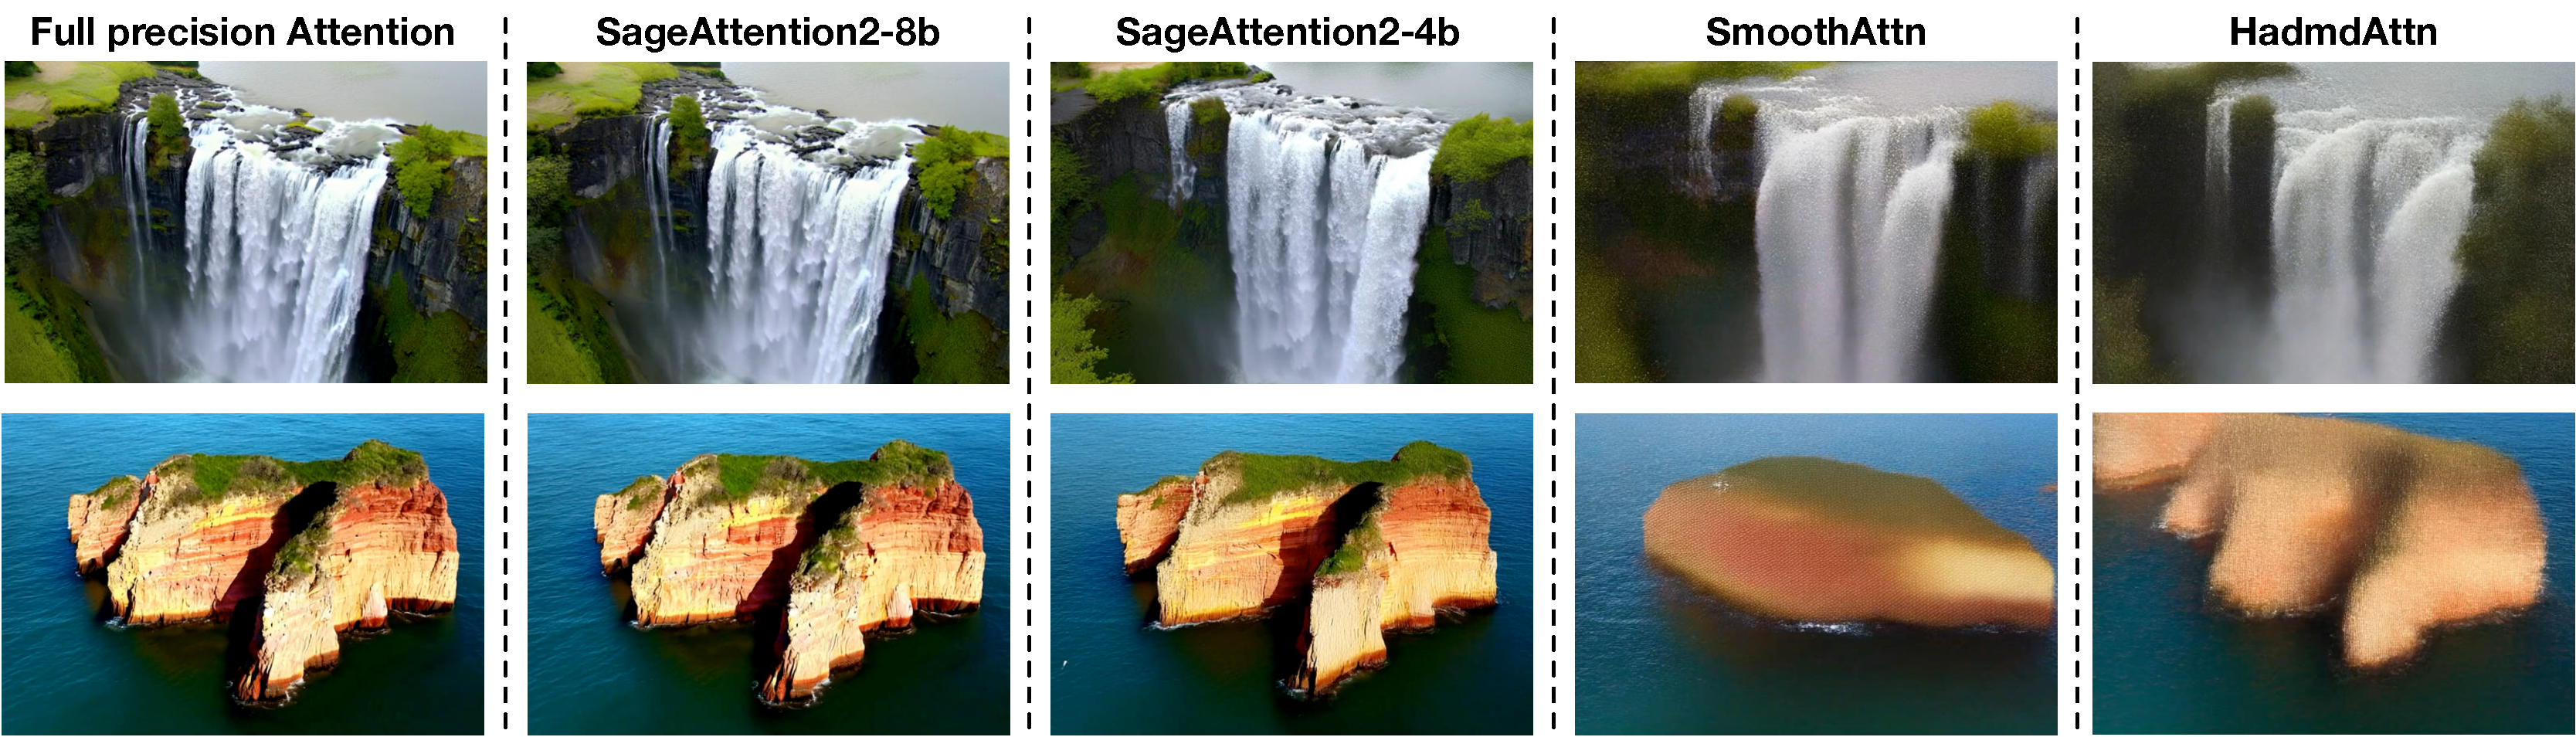
\includegraphics[width=1.0\textwidth]{src/figs/comparison_cogvideo.pdf}
    \vspace{-1em}
    \caption{Comparison examples from \cogvideo(2B), prompts are sampled from open-sora prompt sets.}
    \label{fig:cogvideo2b_example}
    \end{center}
\end{figure}


\begin{figure}[h!]
    \begin{center}
    \includegraphics[width=1.0\textwidth]{src/figs/FA3_example.pdf}
    \vspace{-1em}
    \caption{A comparison example using SageAttn2-8b and FlashAttention3 on \mochi and \hyvideo.}
    \label{fig:video_example}
    \end{center}
\end{figure}



\subsection{Additional Kernel Speed Comparison}  \label{sec:appedix_kernel_speed}
Fig.~\ref{fig:kf_h64_baseline_RTX4090}, ~\ref{fig:kf_h64_baseline_L20}, ~\ref{fig:kf_h128_baseline_L20}, 
~\ref{fig:kf_h64_baseline_H100}, 
~\ref{fig:kf_h128_baseline_H100}, ~\ref{fig:kf_h64_baseline_H20}, and ~\ref{fig:kf_h128_baseline_H20} compare the speed of \our against baselines using headdim=64 and headdim=128, both with and without Causal Mask~\cite{vaswani2017attention}, on RTX4090, L20, H100, and H20 GPUs. 

Table~\ref{tab:speed_comparison_across_gpus} summarizes the performance gain of different attention methods against baselines on various modern GPUs.

\begin{figure*}[h!]
    \centering
    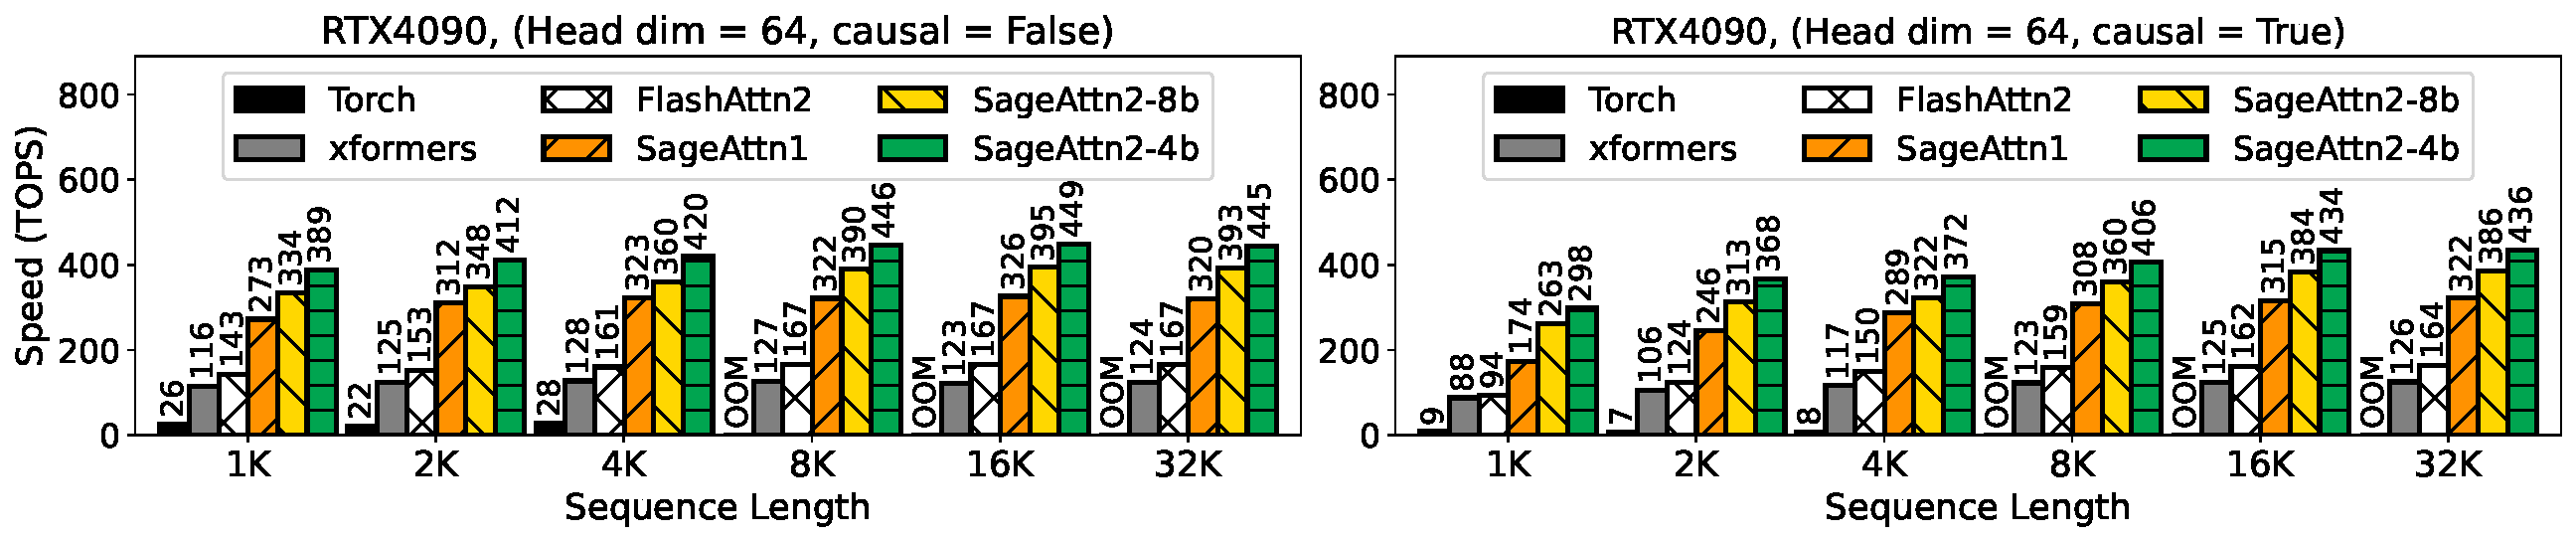
\includegraphics[width=1.0\textwidth]{src/figs/sage_attn2_hd64_baselines_kernel_flops.pdf}
    \vspace{-1em}
    \caption{Speed comparison between \our and baselines (RTX4090, headdim=64).}
    \label{fig:kf_h64_baseline_RTX4090}
\end{figure*}

\begin{figure*}[h!]
    \centering
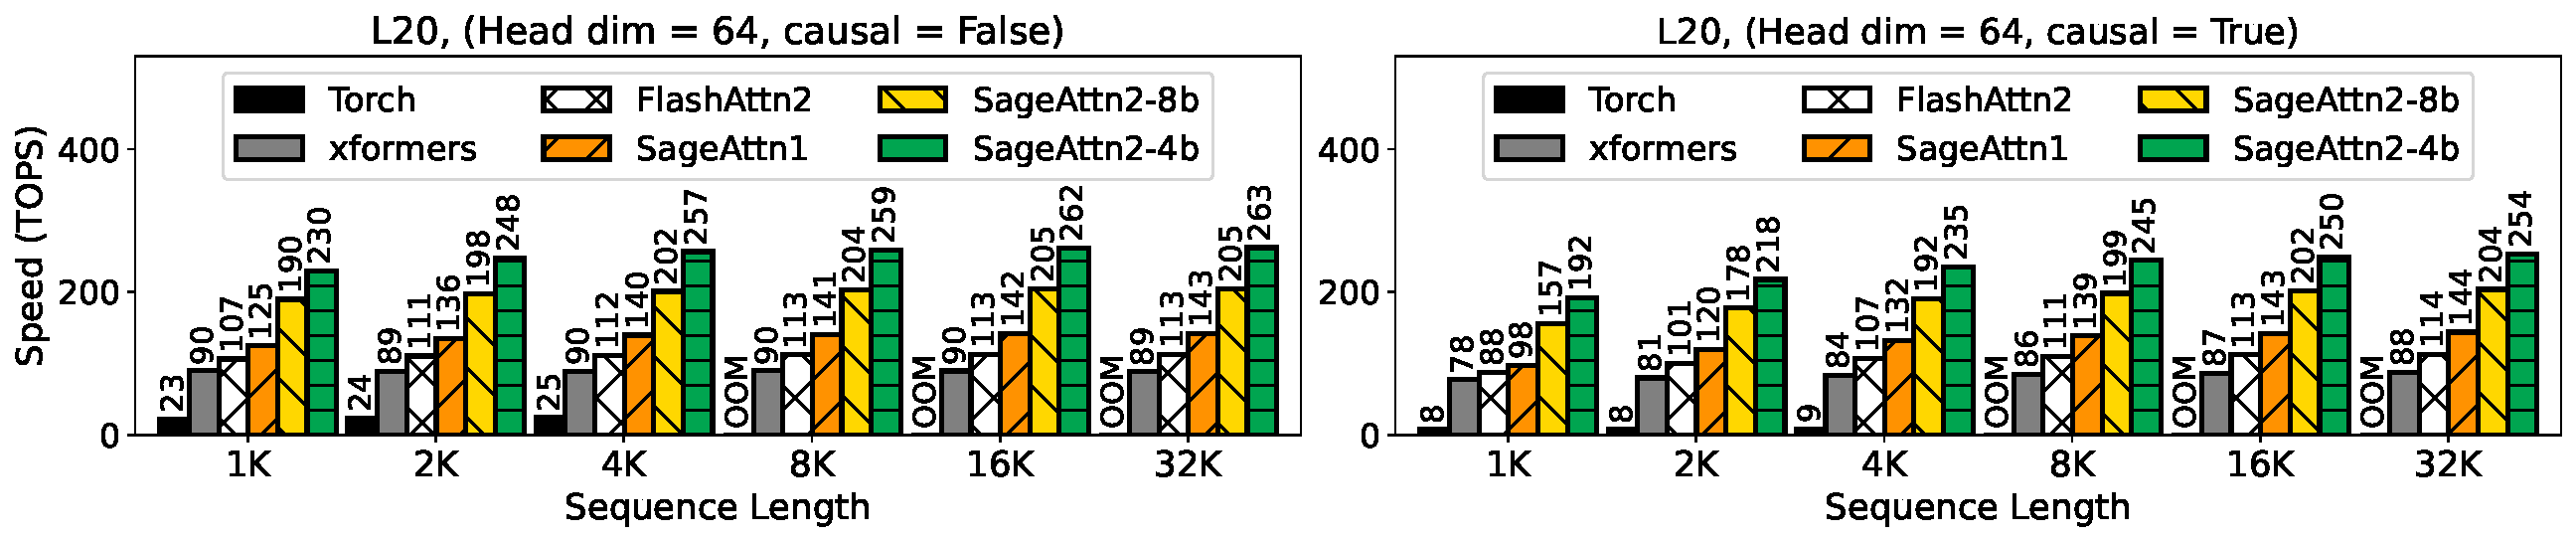
\includegraphics[width=1.0\textwidth]{src/figs/L20sage_attn2_hd64_baselines_kernel_flops.pdf}
\vspace{-1em}
    \caption{Speed comparison between \our and baselines (L20, headdim=64).}
    \label{fig:kf_h64_baseline_L20}
\end{figure*}

\begin{figure*}[h!]
    \centering
    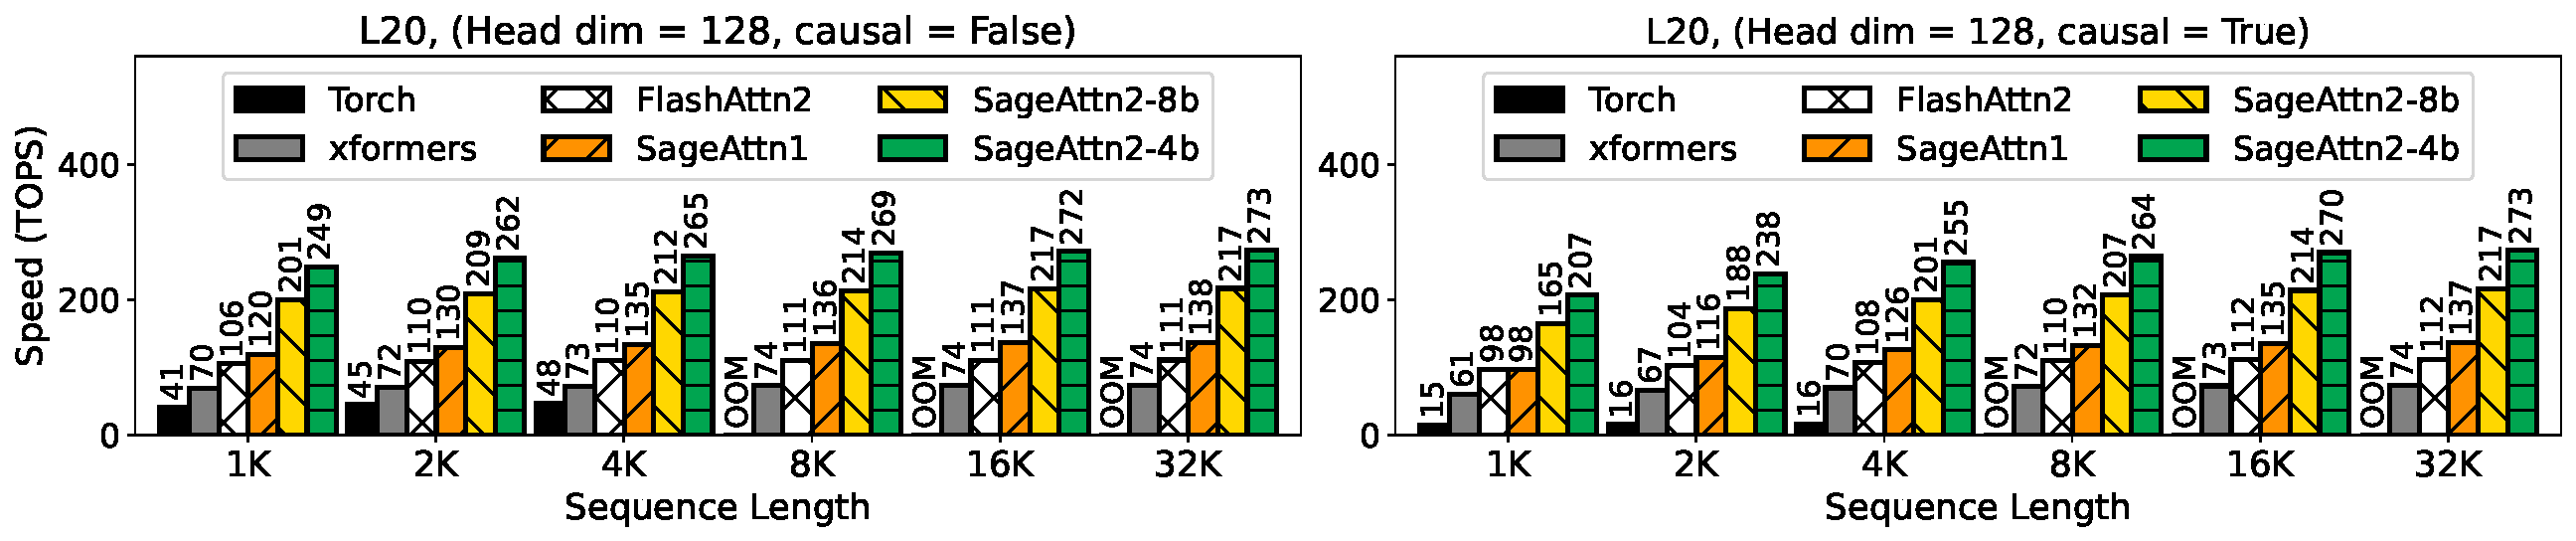
\includegraphics[width=1.0\textwidth]{src/figs/L20sage_attn2_hd128_baselines_kernel_flops.pdf}
    \vspace{-1em}
    \caption{Speed comparison between \our and baselines (L20, headdim=128).}
    \label{fig:kf_h128_baseline_L20}
\end{figure*}


\begin{figure*}[h!]
    \centering
    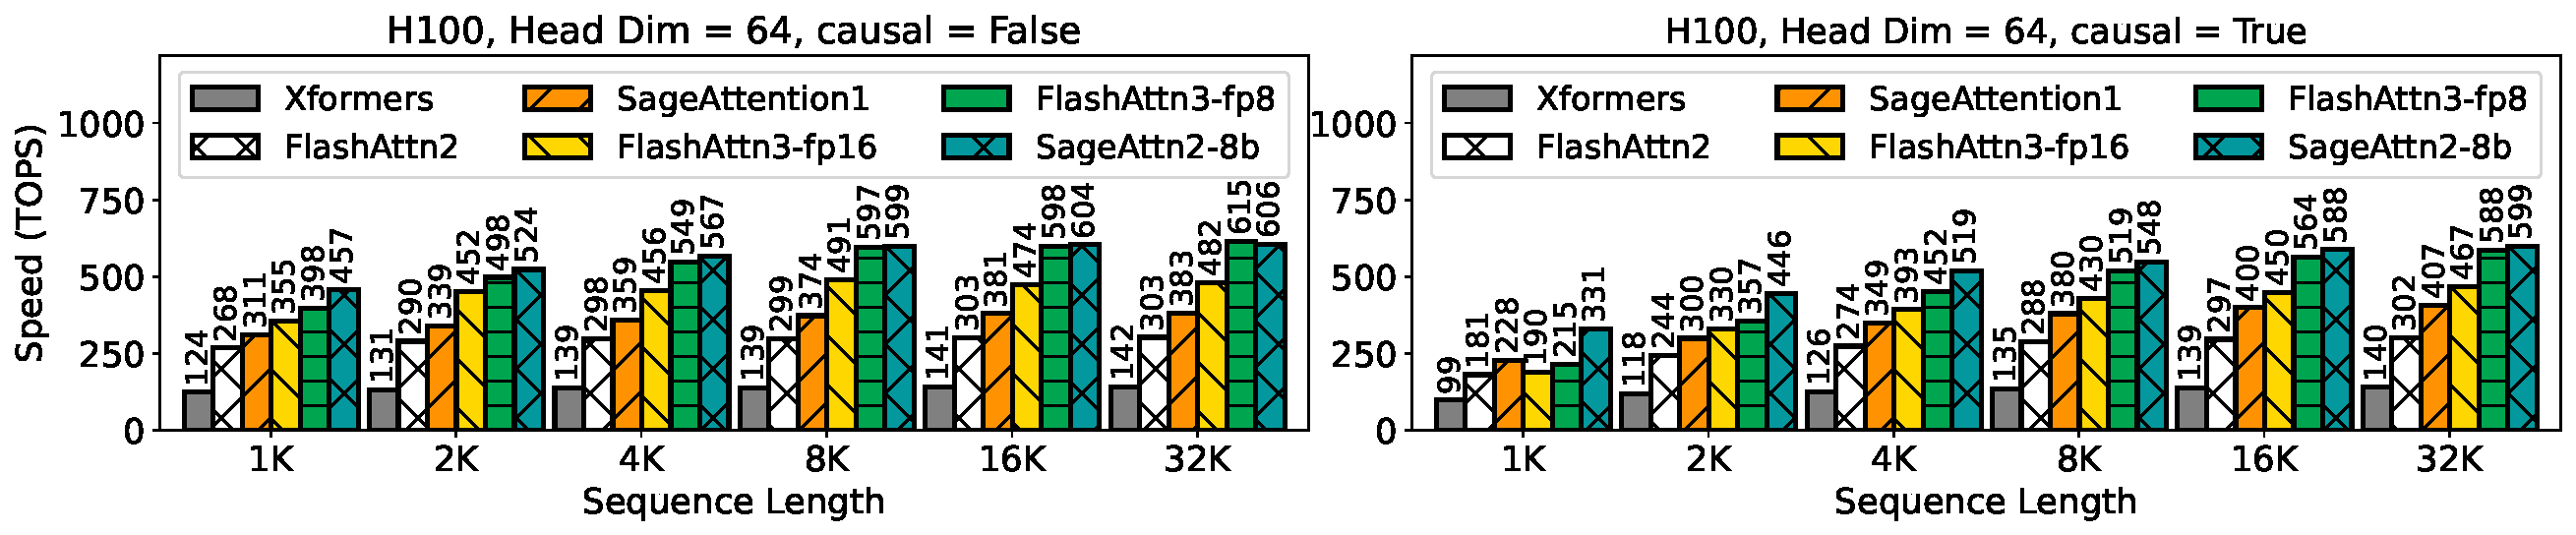
\includegraphics[width=1.0\textwidth]
    {src/figs/H100sage_attn2_hd64_baselines_kernel_flops.pdf}
    \vspace{-1em}
    \caption{Speed comparison between \our and baselines (H100, headdim=64).}
    \label{fig:kf_h64_baseline_H100}
\end{figure*}

\begin{figure*}[h!]
    \centering
    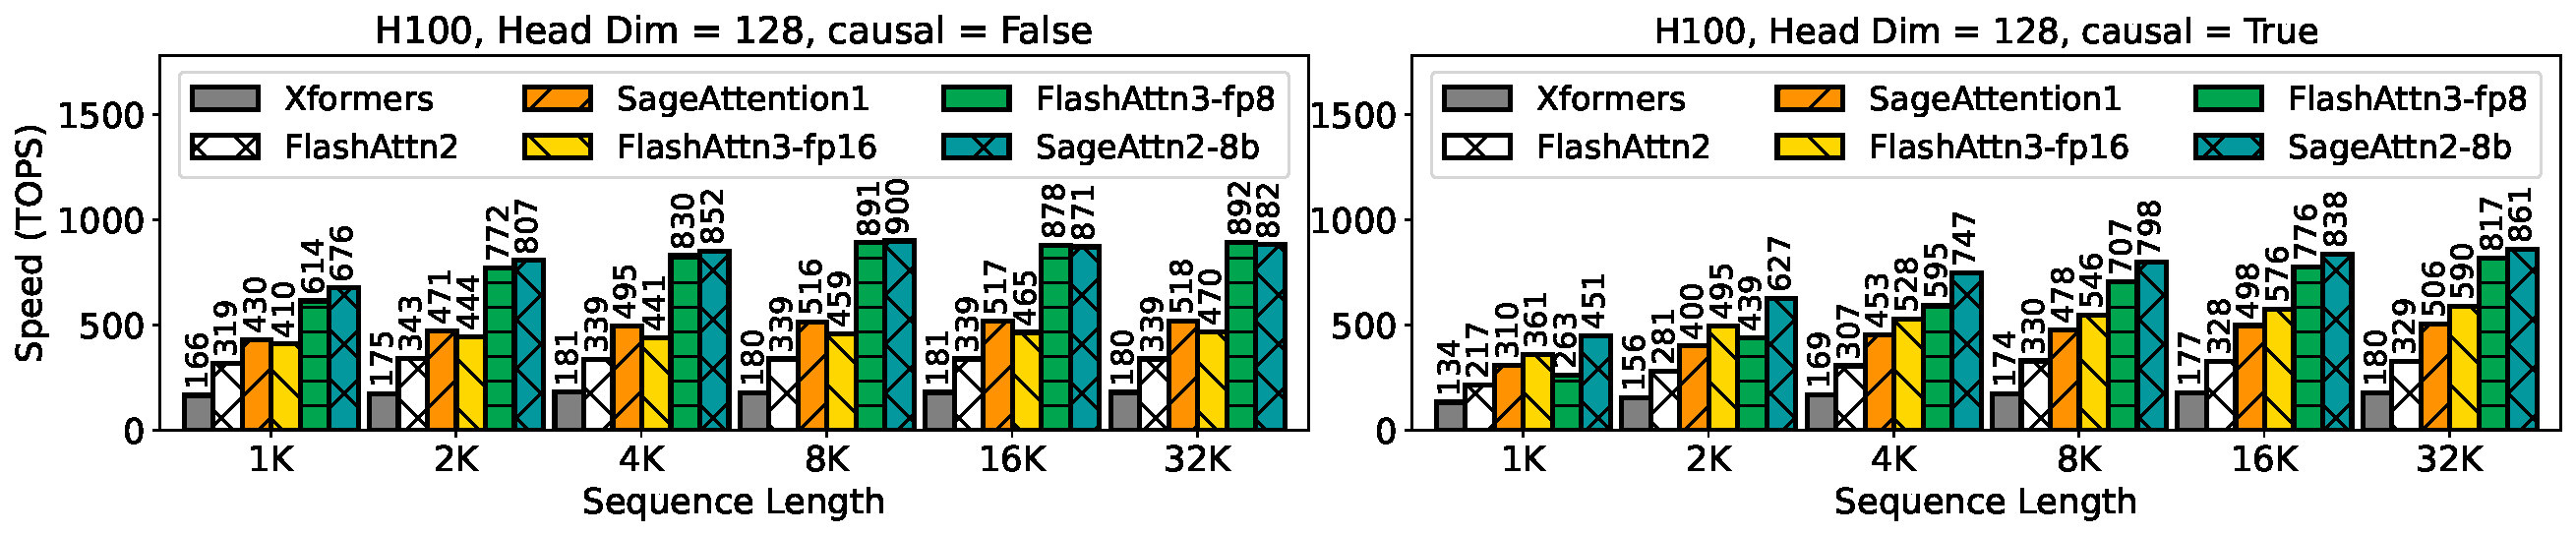
\includegraphics[width=1.0\textwidth]{src/figs/H100sage_attn2_hd128_baselines_kernel_flops.pdf}
    \vspace{-1em}
    \caption{Speed comparison between \our and baselines (H100, headdim=128).}
    \label{fig:kf_h128_baseline_H100}
\end{figure*}

\begin{figure*}[h!]
    \centering
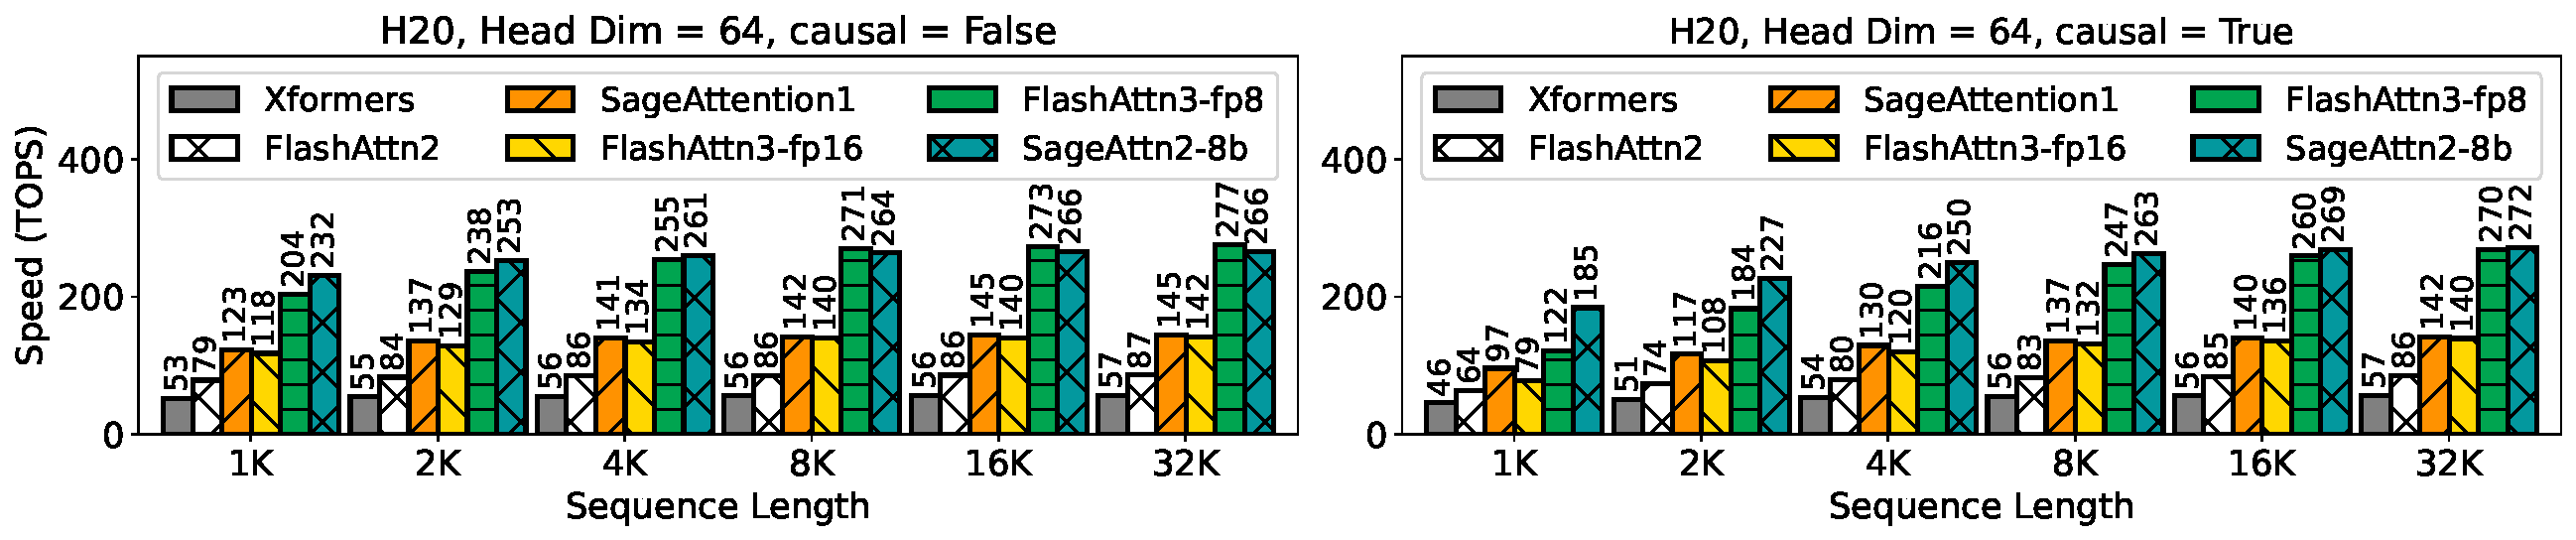
\includegraphics[width=1.0\textwidth]{src/figs/H20sage_attn2_hd64_baselines_kernel_flops.pdf}
\vspace{-1em}
    \caption{Speed comparison between \our and baselines (H20, headdim=64).}
    \label{fig:kf_h64_baseline_H20}
\end{figure*}

\begin{figure*}[h!]
    \centering
    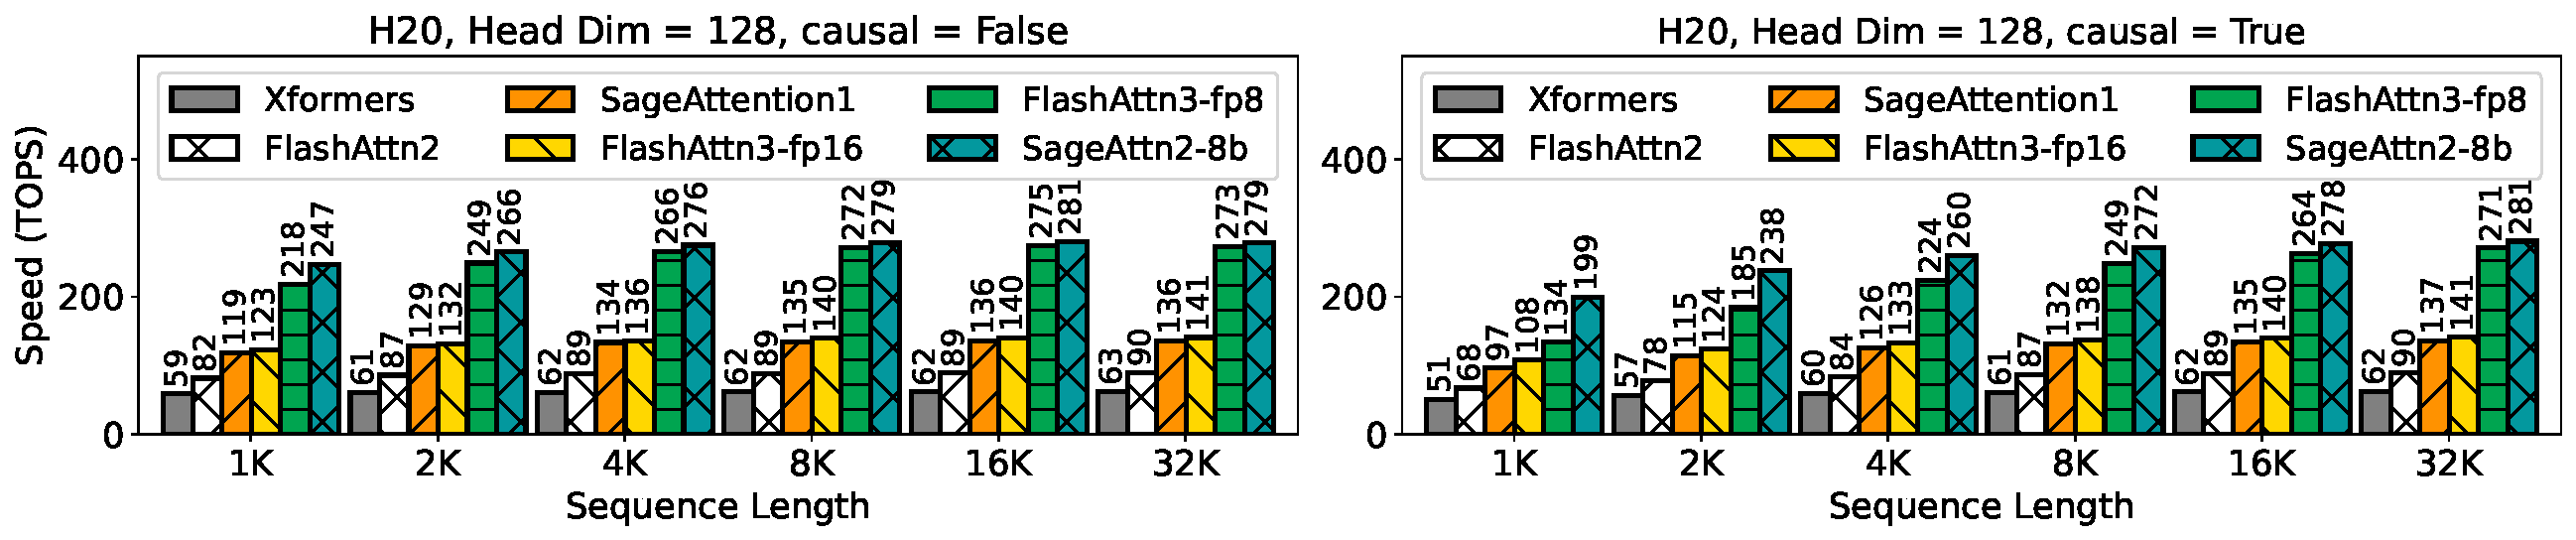
\includegraphics[width=1.0\textwidth]{src/figs/H20sage_attn2_hd128_baselines_kernel_flops.pdf}
    \vspace{-1em}
    \caption{Speed comparison between \our and baselines (H20, headdim=128).}
    \label{fig:kf_h128_baseline_H20}
\end{figure*}


\begin{table*}[h!]
    \centering
    \caption{Speedup of different attention methods on various GPUs.}
    \label{tab:speed_comparison_across_gpus}
    \setlength\tabcolsep{13pt}
    \scalebox{1.0}{
    \begin{tabular}{c|c|c|c|c|c|c|c}
        \toprule
        \textbf{Method} & \textbf{3090} & \textbf{4090} & \textbf{A100} & \textbf{L40} & \textbf{L20} & \textbf{H100} & \textbf{H20} \\
        \midrule
        FlashAttention2 &  1.00  & 1.00 & 1.00 & 1.00 & 1.00 & 1.00 & 1.00 \\
        FlashAttention3 &  \ding{55}  & \ding{55} & \ding{55} & \ding{55} & \ding{55} & 1.37 & 1.57 \\
        FlashAttention3 (fp8) &  \ding{55}  & \ding{55} & \ding{55} & \ding{55} & \ding{55} & 2.63 & 3.06 \\
        SageAttention1  &  1.97  & 1.96 & 1.37 & 1.45 & 1.24 & 1.53 & 1.52 \\
        SageAttention2  &  \ding{55}  & 2.93 & \ding{55} & 2.60 & 2.46 & 2.61 & 3.12 \\
        \bottomrule
    \end{tabular}
    }
    \vspace{-1em}
\end{table*}






\begin{figure}[h!]
    \begin{center}
    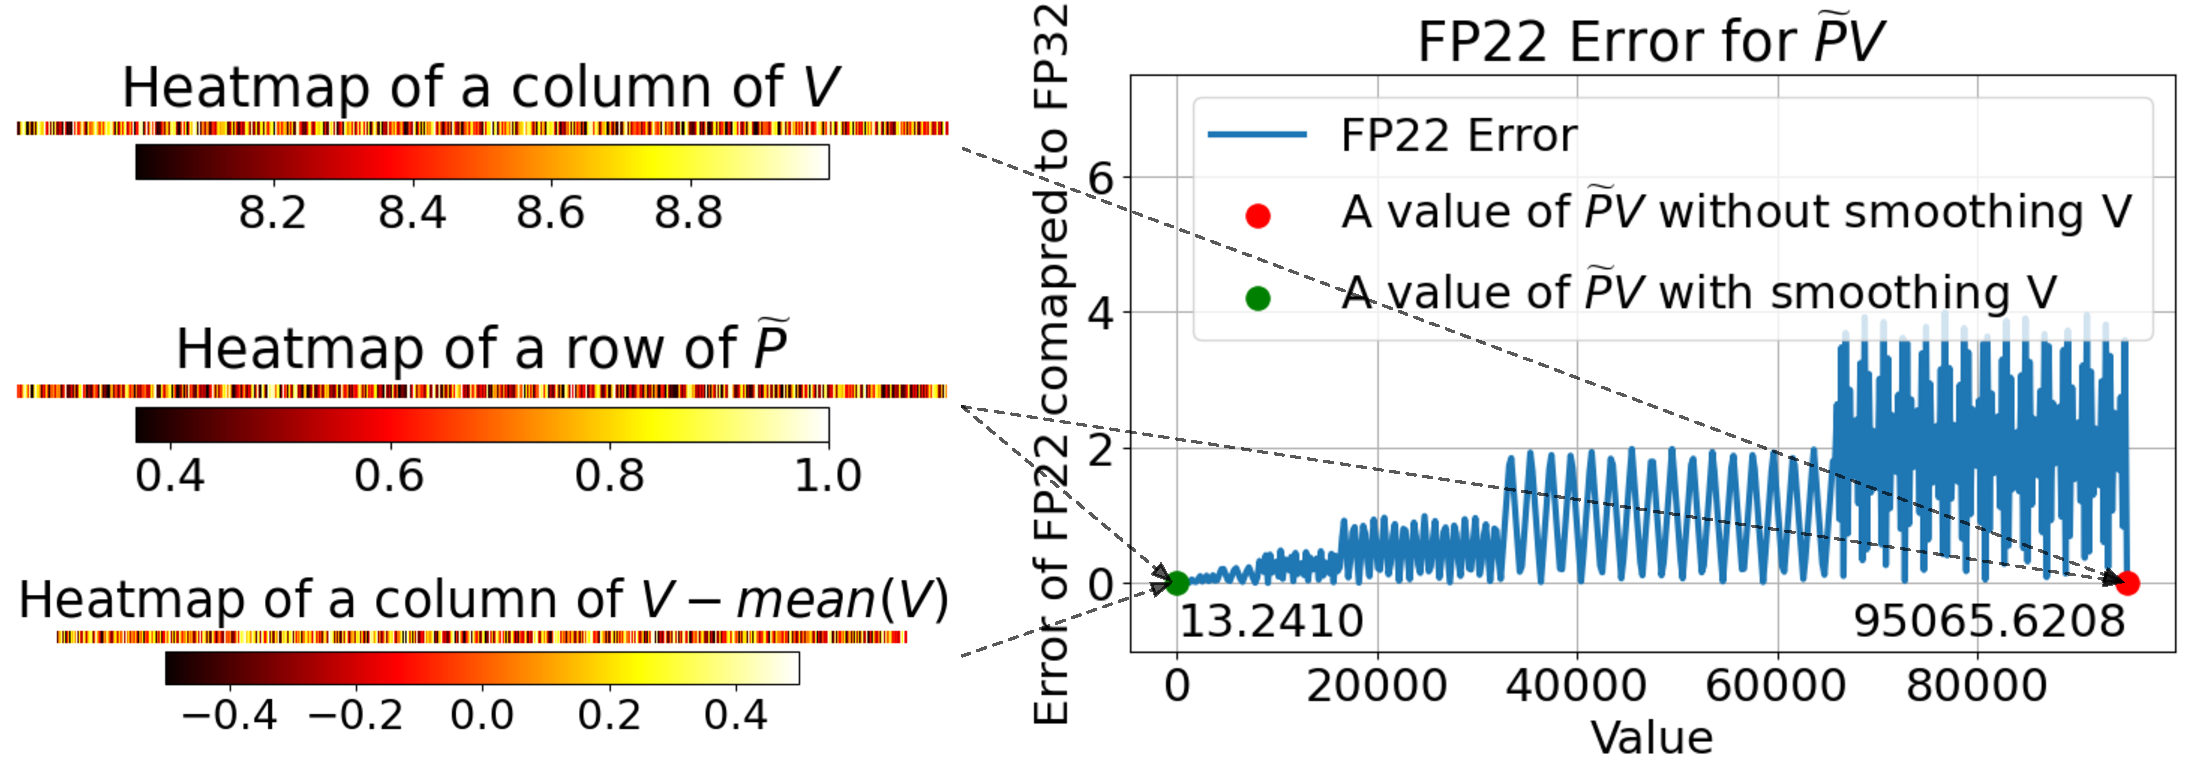
\includegraphics[width=0.69\textwidth]{src/figs/FP22.pdf}
    % \vspace{-1em}
    \caption{An example of dot product precison a row of $\widetilde P$ and a column of $V$ presented by FP22 data type.}
    \label{fig:FP22_precision}
    \end{center}
\end{figure}

\begin{table*}[h!]
    \centering
    \caption{An accuracy example on real tensors of \cogvideo model with or without smoothing $V$.}
    \label{tab:smooth_v1}
        \centering
        \setlength\tabcolsep{12pt}
        \scalebox{1.0}{
        \begin{tabular}{c|c|c|c}
            \toprule
            \textbf{Smooth V} & \textbf{Cos Sim $\uparrow$} & \textbf{Relative L1 $\downarrow$} & \textbf{RMSE $\downarrow$} \\
            \midrule
            \ding{55}          & 98.25\% & 0.1980 & 0.2387 \\
            \checkmark          & \textbf{99.75\%} & \textbf{0.0406} & \textbf{0.0773} \\
            \bottomrule
        \end{tabular}
        }
        \vspace{-1em}
\end{table*}


\subsection{Smoothing V}  \label{sec:appendix_smooth_v}

As shown in Fig.~\ref{fig:FP22_precision}, this strategy could enhance the accuracy of FP22 for values in $\widetilde PV$ for the following reasons: Each row of $\widetilde P$ spans a value range from 0 to 1, and each column of $V$ in some models consistently features channel-wise biases that are exclusively positive or negative, for instance, ranging between 8 and 9 in \cogvideo. Consequently, the values of $\widetilde PV$ could be quite large. However, the floating-point number representation range is not uniform—it is denser near zero. Therefore, by subtracting the mean $\overrightarrow{V_m}$ along the channel dimension from $V$, the values of $\widetilde PV$ will be closer to zero, resulting in a higher representational precision (see Fig.~\ref{fig:FP22_precision} for a visual demonstration).
Additionally, to maintain the correctness of the attention computation, it is only necessary to add $\overrightarrow{V_m}$ to the final calculation of $O$: $O = O + \overrightarrow{V_m}$. This is because the sum of each row of the $\widetilde P$ matrix equals 1, so $\widetilde P\overrightarrow{V_m} = \overrightarrow{V_m}$.
In other words, this method decomposes $V$ into two parts: $\overrightarrow{V_m}$ and $V$. For $V$, it centers the values of each column around zero, which leads to the dot product result between a row from the quantized $\widetilde P$ matrix and a column from the quantized $V$ matrix being closer to zero. This makes the representation of FP22 more accurate. Meanwhile, $\overrightarrow{V_m}$ is retained in FP16 and is added to $O$ at the end without causing a loss of precision for the $\overrightarrow{V_m}$ part.

\subsection{Experiment of Smoothing V}  \label{sec:exp_of_smooth_v}
Table~\ref{tab:smooth_v1} shows the attention accuracy on real tensors sampled from \cogvideo with and without smoothing $V$. It demonstrates that smoothing $V$ could improve the accuracy of \our when quantizing $Q, K$ to INT4 and $\widetilde P, V$ to FP8. We find that smoothing V is generally effective for diffusion models~\cite{zheng2023dpm,zheng2024diffusion,zheng2024masked,zheng2025direct,zhao2024identifying,zhao2025riflex,wang2024framebridge}.

\subsection{Theoretical Analysis of Smoothing}  \label{sec:smoothing_theoretical}
In this section, we analyze the benefit of smoothing from a theoretical perspective. Let $X \in \mathbb{R}^{N \times d}$ be $N$ activation tokens of dimension $d$. Following \cite{dettmers2023qlora},  we suppose that an activation token follows an Gaussian distribution $\mathcal{N}(\boldsymbol{\mu}, \Sigma^2)$, where $\boldsymbol{\mu} = (\mu_1, \mu_2, \ldots, \mu_d)$ and $\Sigma^2$ is a diagonal matrix with $\Sigma^2 = \mathrm{diag}(\sigma_1^2, \sigma_2^2, \ldots, \sigma_d^2)$. Further, we suppose that different token $X_i$ is i.i.d. sampled from the same distribution.

Suppose the absolute maximum value in a quantization group~\cite{hu2025quant,zhang2025int8train} is $M$, and the bit width is $b$, then there are $2^b$ quantization levels. Under the round-to-nearest strategy, the expected quantization error is $\frac{1}{2} \cdot \frac{2M}{2^b}$, which is proportional to the maximum absolute value in the quantization group. So a smaller absolute maximum value leads to smaller quantization error.

After smoothing, we have: 
\begin{equation}
   Y_{ij} = X_{ij} - \frac{1}{N} \sum_{k=1}^N X_{kj} 
\end{equation}
and $Y_{ij}$ also follows a Gaussian distribution. The mean and variance of $Y_{ij}$ can be calculated as follows:
\begin{align}
\mathbb{E}[Y_{ij}] &= \mathbb{E}[X_{ij}] - \frac{1}{N} \sum_{k=1}^N \mathbb{E}[X_{kj}] = \mu_j - \frac{1}{N} \sum_{k=1}^N \mu_j = 0 \\
\mathrm{Var}[Y_{ij}] &= \mathrm{Var}[\frac{N-1}{N} X_{ij}] + \sum_{k=1, k\neq i}^N \mathrm{Var}[\frac{1}{N} X_{kj}] = \frac{(N-1)^2}{N^2} \sigma_j^2 + (N-1) \frac{1}{N^2} \sigma_j^2 = \frac{(N-1)}{N} \sigma_j^2
\end{align}
So $Y_{ij}$ has a smaller mean and variance compared to $X_{ij}$. Following the property of Gaussian distribution, we have: 
\begin{equation}
    P(|Y_{ij}| < \epsilon) > P(|X_{ij}| > \epsilon),\ \forall \epsilon > 0
\end{equation}
So the distribution of $X_{ij}$ is more concentrated toward 0 after smoothing. Then we know that
\begin{equation}
    P(\mathrm{absmax}(Y_i) < \epsilon) = \prod_{j=1}^d P(|Y_{ij}| < \epsilon) > \prod_{j=1}^d P(|X_{ij}| > \epsilon) = P(\mathrm{absmax}(X_i) < \epsilon)\
\end{equation}
So this makes the distribution of absolute max value in a token more concentrated towards 0, leading to smaller quantization error.



\subsection{Per-Thread Quantization Formulation}  \label{sec:per_thread_formulation}

\begin{figure}[h!]
    \begin{center}
    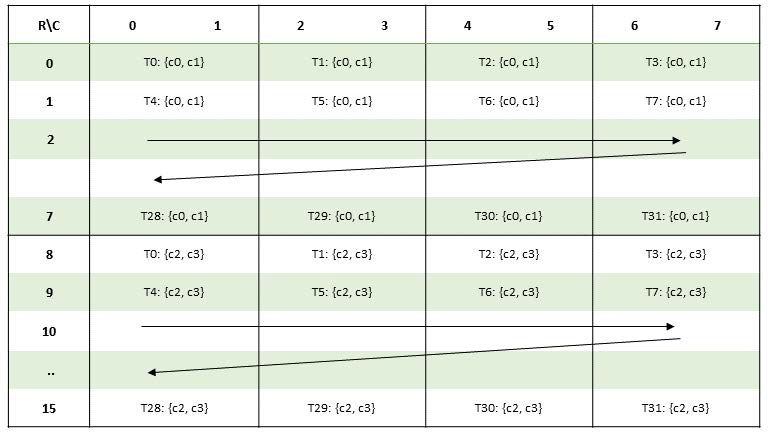
\includegraphics[width=0.69\textwidth]{src/figs/tensor_core.jpg}
    % \vspace{-.6em}
    \caption{Memory layout of INT4/INT8 tensor core for accumulator matrix $C$ and $D$ in $D=A*B+C$ among 32 threads (T0 $\sim$ T31) in a warp. $C$ and $D$ is of shape 16x8. Each thread only holds 4 out of the 128 elements.}
    \label{fig:tensor_core_layout}
    \end{center}
\end{figure}

To further clarify the per-thread quantization, we first introduce the INT4 MMA instruction of Tensor Core, and then give the formulation of per-thread quantization.

Tensor cores, first introduced in NVIDIA's Volta architecture, are specialized units designed for efficient matrix-multiply-and-accumulate (MMA) operations. Their usage significantly enhances computational efficiency and performance in AI and high-performance computing (HPC) workloads.
Tensor cores compute small tiles of MMA operations, specifically $D = A * B + C$ on a warp (32 contiguous threads) basis. Each thread in the warp holds a fragment of input matrices and will get a fragment of output matrix as a computation result. The INT4 \texttt{mma.m16n8k64} tensor core operation computes the product of a $16\times64$ INT4 matrix $A$ and a $64\times8$ INT4 matrix $B$, both stored in registers. It accumulates the result into a $16\times8$ INT32 matrix $C$, also stored in registers, and returns the final product matrix $D$, which has the same shape ($16\times8$), data type (INT32), and storage location (registers). Each thread holds only $\frac{1}{32}$ of the input and output data. Fig.~\ref{fig:tensor_core_layout} extracted from the PTX document~\cite{ptx} shows the memory layout of matrix $C$ and $D$ among 32 threads in a warp. Each thread only holds 4 out of the 128 result elements.

% \noindent\textbf{Per-Thread Quantization.}

\begin{align}  \label{equ:per_thread_quant}
    i_{\delta q} =& \lfloor (n*8*c_w/b_q) \rfloor \notag \\
    q_i[i_{\delta q}] =& \{ 8\times(n\%8) + \lfloor (n*\frac{c_w}{b_q}) \rfloor * \frac{b_q}{c_w}\}  , ~  n \in [0, N]  \notag \\
    \delta_{Q}[i_{\delta q}] =& \frac{\max(\left|\,Q[q_i[i_{\delta q}]]\,\right|)}{7} \notag \\ \notag
    \hat Q[q_i[i_{\delta q}]] =& \left\lceil \frac{Q[q_i[i_{\delta q}]]}{\delta_{Q}[i_{\delta q}]} \right\rfloor \\ 
    i_{\delta k} =& \lfloor (n*4/b_{k}) \rfloor  \\ \notag
    k_n[i_{\delta k}] =& \{ 8\times(n\%8) + \lfloor n/b_{k} \rfloor * b_{k} \} \cup \\ &\{ 8\times(n\%8)+1 + \lfloor n/b_{k} \rfloor * b_{k}\}   , ~~  n \in [0, N]  \notag \\
    \delta_{K}[i_{\delta k}] =& \frac{\max(\left|\,K[k_n[i_{\delta k}]]\,\right|)}{7} \notag \\ \notag
    \hat K[k_n[i_{\delta k}]] =& \left\lceil \frac{K[k_n[i_{\delta k}]]}{\delta_{K}[i_{\delta k}]} \right\rfloor
\end{align}


By ensuring results held by each thread share a common dequantization scale (belong to the same quantization group), we can avoid the overhead associated with per-token quantization. Leveraging this observation, we design per-thread quantization as formulated in Eq.~\ref{equ:per_thread_quant}, where $c_w$ is the count of GPU Warps, $b_q$ and $b_k$ are the block size of $Q, K$, and $n$ is the token index of $Q, K$.
% as shown in Fig.~\ref{fig:per_thread}. 
For typical block size of $b_q=128$, $b_k=64$ and warp number $c_w=4$ (as used in FlashAttention2), each warp processes a tile of 32 query tokens and 64 key tokens. Query tokens $i,8+i,16+i,24+i$ ($i = 0,1,\cdots,7$) can be made into one quantization group and key tokens $j,1+j,8+j,9+j,\cdots,56+j,57+j$ ($j=0,1,2,3$) can be made into one quantization group, as visualized in Fig.~\ref{fig:per_thread}. This design aligns with the memory layout of output matrix $D$ of tensor core shown in Fig.~\ref{fig:tensor_core_layout}, ensuring that each thread only needs one $Q$ scale and one $K$ scale for dequantization.

As a result, this approach creates 32 quantization groups for $Q$ (8 for each of the 4 warps) and 4 quantization groups for $K$ in a 128x64 block, providing $32\times$ and $4\times$ finer granularity compared to per-block quantization for query tokens and key tokens, respectively. Table~\ref{tab:quant_granularities1} and Table~\ref{tab:quant_granularities2} show the accuracy gains by using per-thread quantization. Per-thread quantization achieves accuracy that closely matches per-token quantization, without introducing any kernel speed degradation (see Table~\ref{tab:ablation_overhead_smoothing} and \ref{tab:granularity_speed_ablation}). 






\subsection{Datasets and Metrics in Experiments}  \label{sec:exp_dataset_metrics}

\noindent \noindent\textbf{Datasets.}   
Text-to-text models are evaluated on four zero-shot tasks: WikiText~\cite{merity2022pointer} to assess the model's prediction confidence, LAMBADA~\cite{paperno2016lambada} evaluate contextual understanding, MMLU~\cite{2020mmlu} for measuring knowledge across various subjects, and Longbench~\cite{bai2023longbench} for comprehensive assessment of long context understanding capabilities.
Text-to-video models are evaluated using the open-sora~\cite{opensora} prompt sets.
Text-to-image models are assessed on MJHQ-30K~\cite{li2024playground}.
\timm is evaluated on on three image datasets: ImageNet~\cite{deng2009imagenet}, ImageNet-Sketch (Sketch)~\cite{wang2019sketch}, and ImageNet-Rendition (ImageNet-r)~\cite{hendrycks2021rendition}. 

\noindent \noindent\textbf{End-to-end metrics.}   
For text-to-text models, we use perplexity (ppl.)~\cite{jelinek1977perplexity} for WikiText, Accuracy (Acc.) for LAMBADA and MMLU, and Longbench score~\cite{bai2023longbench}.
For text-to-video models, following~\citet{zhao2024viditq}, we evaluate the quality of generated videos on five metrics: CLIPSIM and CLIP-Temp (CLIP-T)~\cite{liu2024evalcrafter} to measure the text-video alignment; (VQA-a) and (VQA-t) to assess the video aesthetic and technical quality, respectively; and Flow-score (FScore) for temporal consistency~\cite{wu2023exploring}. 
For text-to-image models, generated images are compared with the images in MJHQ-30K dataset in three aspects: FID~\cite{heusel2017gans} and sFID~\cite{salimans2016improved} for fidelity evaluation, \textit{Clipscore} (CLIP)~\cite{hessel2021clipscore} for text-image alignment, and \textit{ImageReward} (IR)~\cite{xu2024imagereward} for human preference.
For \timm, we use classification accuracy.

\noindent\textbf{Accuracy metrics.} We use three metrics to assess the accuracy of quantized attention output $O'$ compared to attention output in full-precision $O$: First, we flatten $O'$ and $O$ into vectors in the shape of $1\times n$. Then, Cosine similarity: $CosSim=\sum OO' / \smash{\sqrt{\sum O^2}} \smash{\sqrt{\sum O'^2}}$, Relative L1 distance: $L1=\sum |O - O'| / \sum |O|$, Root mean square error: $RMSE=\sqrt{(1/n) \sum (O - O')^2}$.

\subsection{Kernel Benchmark Setup}  \label{sec:kernel_benchmark_setting}
We benchmark kernel speed with a batch size of 4 and 32 attention heads across a variety of sequence lengths. Benchmarks are conducted using head dimensions of 64 and 128, both with and without Causal Mask~\cite{vaswani2017attention}. To generate input tensors for benchmarking, we follow standard practices adopted in prior works such as FlashAttention~\cite{dao2022flashattention}. For floating-point data types, inputs are drawn from a Gaussian distribution with mean 0 and standard deviation 1, while for integer data types, inputs are uniformly sampled within the representation range:[-128, 127] for INT8 and [-8, 7] for INT4.

\begin{table*}[h!]
    \caption{End-to-end metrics on \llama (7B).}
    \label{exp:metrics_loss_t2t-appendix}
    \setlength\tabcolsep{5.5pt}
    \begin{center}
    \scalebox{1.0}{\begin{tabular}{p{2.12cm}|p{3cm}|c|c|c}
    \toprule
    {\bf Model}  & {\bf Attention}  & {\bf WikiText (Ppl.) $\downarrow$}  & {\bf Lambda (Acc.) $\uparrow$}  & {\bf MMLU (Acc.) $\uparrow$}  \\ \hline
    \multirow{6}{*}{\llama} & Full-Precision & 5.823 & 0.886  & 0.439    \\  
    & \texttt{HadmdAttn} & 6.771 &  0.860 &  0.360 \\
    & \texttt{SmoothAttn} & 6.717 &  0.867 & 0.392  \\
    & \texttt{SageAttention} & \textbf{5.824} &  \textbf{0.887}  & \textbf{0.439}  \\
    & \ourf & \textbf{5.912} &  \textbf{0.881}  &  \textbf{0.428}   \\ 
    & \oure & \textbf{5.828} &  \textbf{0.886}  & \textbf{0.438} \\ 
    \bottomrule
    \end{tabular} }
    \end{center}
    \vspace{-1em}
\end{table*}


\begin{table*}[h!]
    \caption{End-to-end metrics on \cogvideo (2B).}
    \label{exp:metrics_loss_cogvideo2b-appendix}
    \setlength\tabcolsep{7.2pt}
    \begin{center}
    \scalebox{1.0}{\begin{tabular}{p{2.12cm}|p{3cm}|c|c|c|c|c}
    \toprule
    {\bf Model}  & {\bf Attention}  & {\bf CLIPSIM $\uparrow$}  & {\bf CLIP-T $\uparrow$}  & {\bf VQA-a $\uparrow$}  & {\bf VQA-t $\uparrow$}  & {\bf FScore $\uparrow$} \\ \hline
    \multirow{6}{*}{\hspace{-.75em}\makecell[c]{\cogvideo\\(2B)}} & \hspace{-.3em}Full-Precision  & 0.1836 & 0.9975  & 77.605  &  75.360  &  3.006 \\ 
    & \hspace{-.3em}\texttt{HadmdAttn} & 0.1742 & 0.9877  & 29.780  & 23.985   & 0.499  \\
    & \hspace{-.3em}\texttt{SmoothAttn} & 0.1741 & 0.9870  & 41.703  & 47.043   &  0.624  \\
    & \hspace{-.3em}\texttt{SageAttention}  & \textbf{0.1833} &  \textbf{0.9976}  &  \textbf{76.997}  &  \textbf{71.360}  & \textbf{2.988} \\
    & \hspace{-.3em}\ourf  & \textbf{0.1821} &  \textbf{0.9973}  &  \textbf{77.368}  &  \textbf{74.906} & \textbf{2.603} \\ 
    & \hspace{-.3em}\oure  & \textbf{0.1829} &  \textbf{0.9977}  &  \textbf{76.532}  &  \textbf{74.281}  & \textbf{2.941}  \\
    \bottomrule
    \end{tabular} }
    \end{center}
    \vspace{-1em}
\end{table*}


\begin{table*}[h!]
    \caption{End-to-end metrics on an image classification model.}
    \label{exp:metrics_loss_t2t-3_appendix}
    \begin{center}
    \setlength\tabcolsep{10pt}
    \scalebox{1.0}{\begin{tabular}{p{1.58cm}|p{2.7cm}|c|c|c}
    \toprule
    {\bf Model}  & {\bf Attention}  & {\bf ImageNet (Acc.) $\uparrow$}  & {\bf Sketch (Acc.) $\uparrow$}  & {\bf ImageNet-r (Acc.) $\uparrow$}  \\ \hline
    \multirow{6}{*}{\timm} & \hspace{-.3em}Full-Precision  & 84.79\% & 45.32\%  & 59.55\%   \\ 
    & \hspace{-.3em}\texttt{HadmdAttn}  & 84.50\% & 44.89\%  &  58.80\%   \\
    & \hspace{-.3em}\texttt{SmoothAttn}  & 84.40\% &  44.68\% &  58.73\%  \\
    & \hspace{-.3em}\texttt{SageAttention} & \textbf{84.74\%}  & \textbf{45.38\%}  & \textbf{59.95\%}   \\
    & \hspace{-.3em}\ourf & \textbf{86.67\%}  & \textbf{45.24\%}  & \textbf{59.29\%}   \\
    & \hspace{-.3em}\oure & \textbf{84.79\%}  & \textbf{45.39\%}  & \textbf{59.57\%}   \\
     \bottomrule
    \end{tabular} }
    \end{center}
    \vspace{-1em}
\end{table*}


\begin{table*}[h!]
    \caption{Comparison with FlashAttention3(fp8) on \texttt{Llama-3-262k} (8B) on InfiniBench~\cite{zhang-etal-2024-bench} (H100 GPU).}
    \label{exp:infinibench_llama3_262k_appendix}
    \begin{center}
    \setlength\tabcolsep{5pt}
    \scalebox{0.85}{\begin{tabular}{p{2.8cm}|c|c|c|c|c|c|c|c|c}
    \toprule
    {\bf Attention}  & {\bf Eng.Sum}  & {\bf Eng.QA} & {\bf Eng.MC}  & {\bf Code.Debug} &{\bf Math.Find} & {\bf Retr.PassKey} & {\bf Retr.Num} & {\bf Retr.KV} & {\bf Avg.}  \\ \hline
    Full-Precision  & 18.03 & 12.5 & 64.19 &  24.37 & 18.29 & 100.0 & 100.0 & 7.0 & 43.05\\ 
    \texttt{FlashAttn3-fp8}  & \textbf{19.03} & 11.73  & 55.90 & 22.59 & \textbf{22.57} & \textbf{100.0} & \textbf{100.0} & 0.4 & 41.53\\
    \our  & 18.17 &  \textbf{12.46} & \textbf{64.19} & 2\textbf{5.63} & 17.43 & \textbf{100.0} & \textbf{100.0} & \textbf{6.6} & \textbf{43.06}\\
    \bottomrule
    \end{tabular}}
    \end{center}
    \vspace{-1em}
\end{table*}

\begin{figure}[h!]
    \centering
    \subfigure[Full Precision]{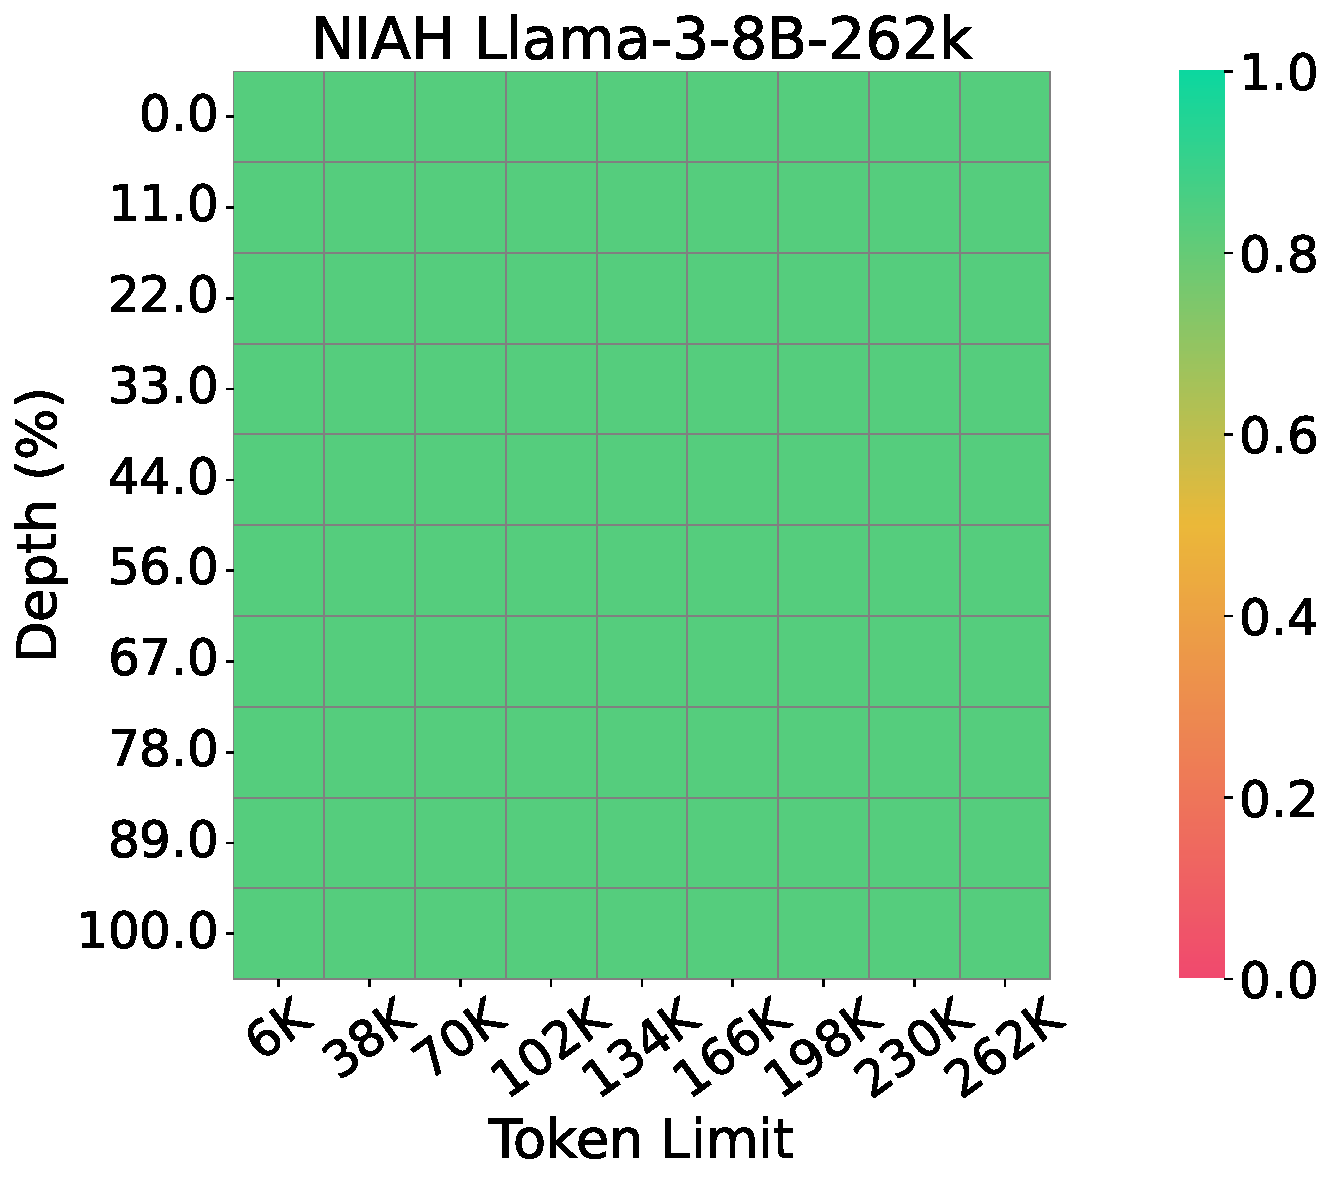
\includegraphics[width=0.3\textwidth]{src/figs/niah_llama-3-8b-262k-fa3.pdf}}
    \subfigure[\texttt{FlashAttn3-fp8}]{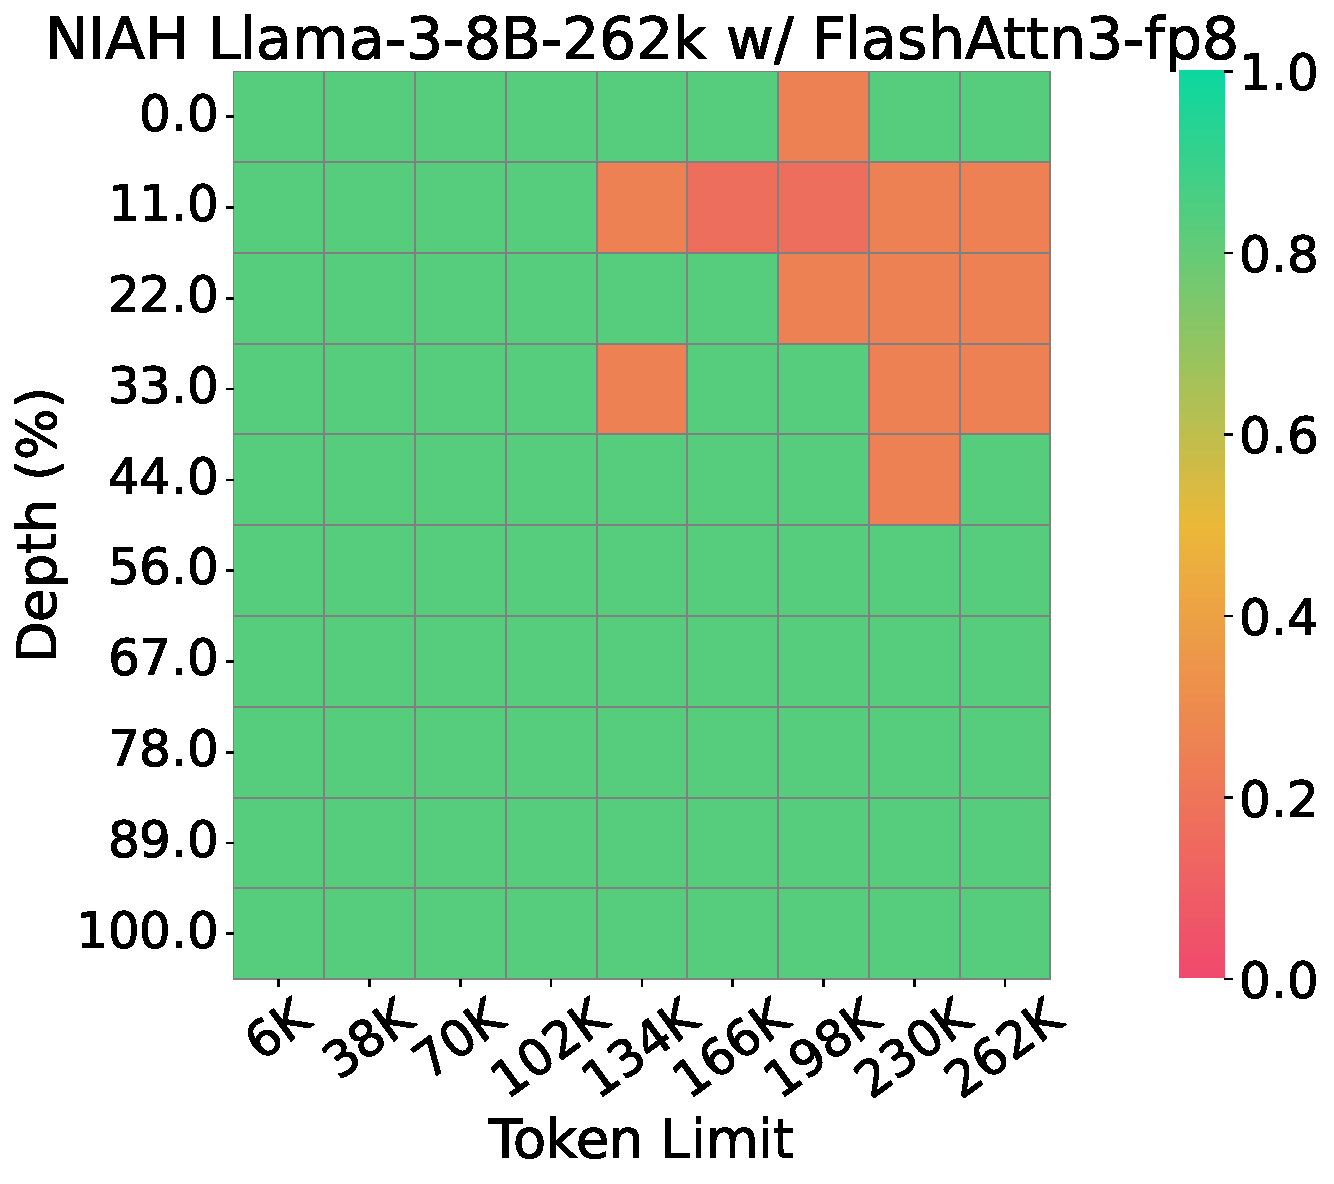
\includegraphics[width=0.3\textwidth]{src/figs/niah_llama-3-8b-262k-fa3-fp8_fa3_fp8.pdf}}
    \subfigure[\our]{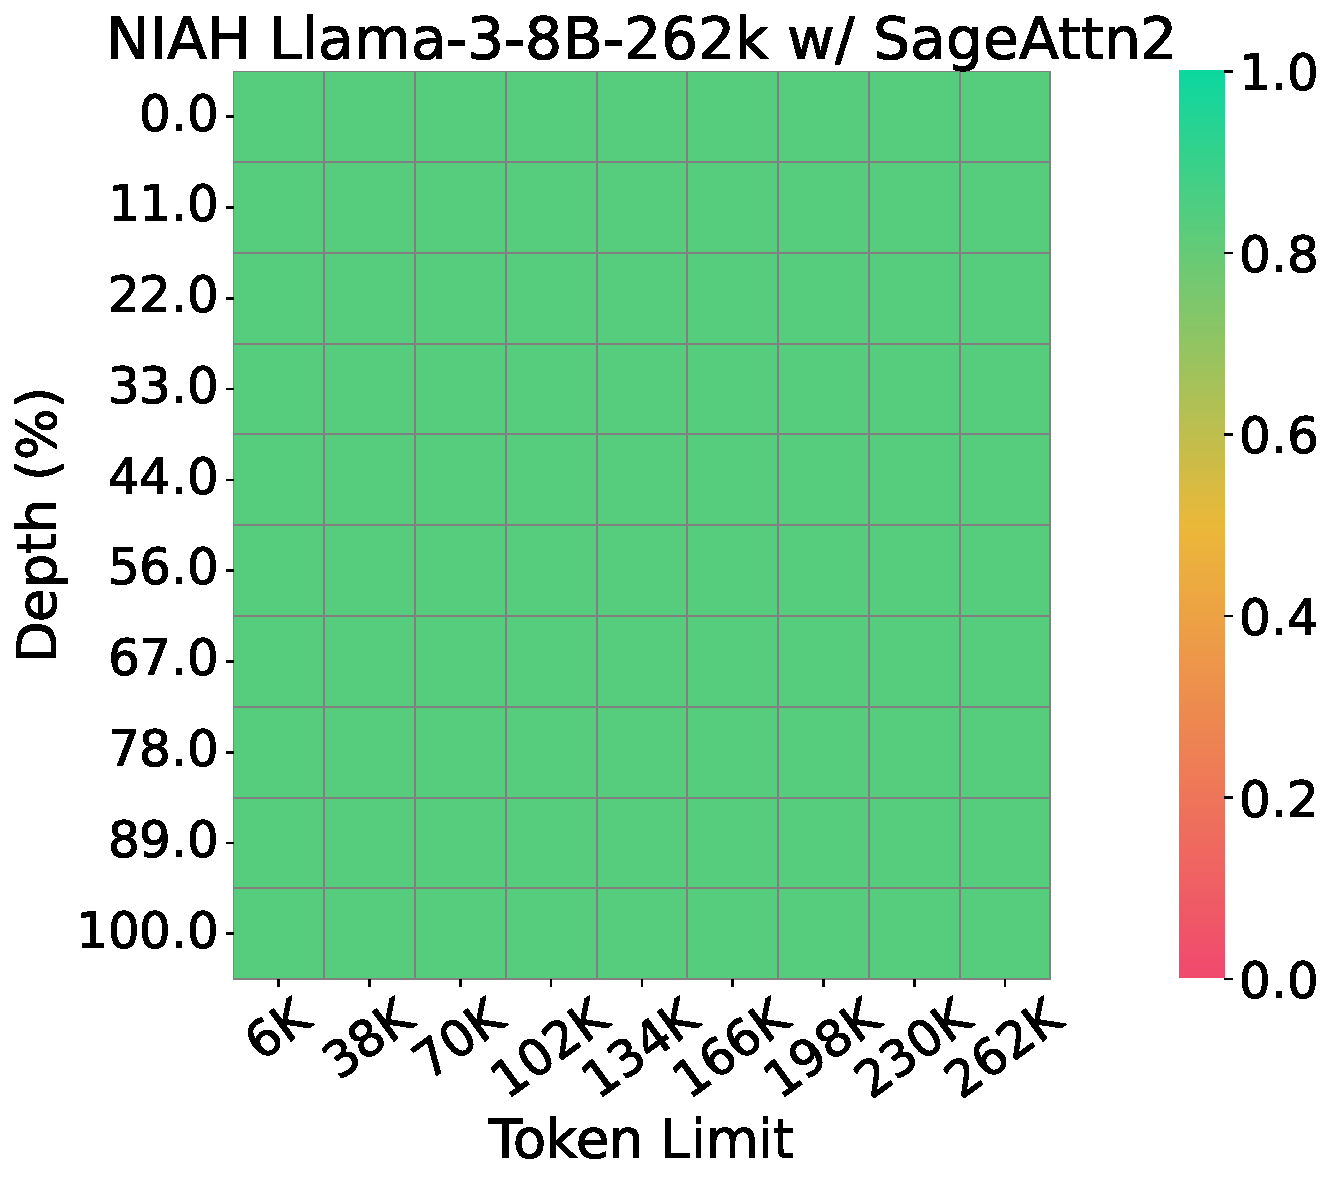
\includegraphics[width=0.3\textwidth]{src/figs/niah_llama-3-8b-262k_sage2.pdf}}
    \vspace{-1em}
    \caption{Needle In A Haystack results on \texttt{Llama-3-262k} (8B).}
    \label{fig:llama3_262k_niah}
\end{figure}

\begin{figure}[h!]
    \begin{center}
    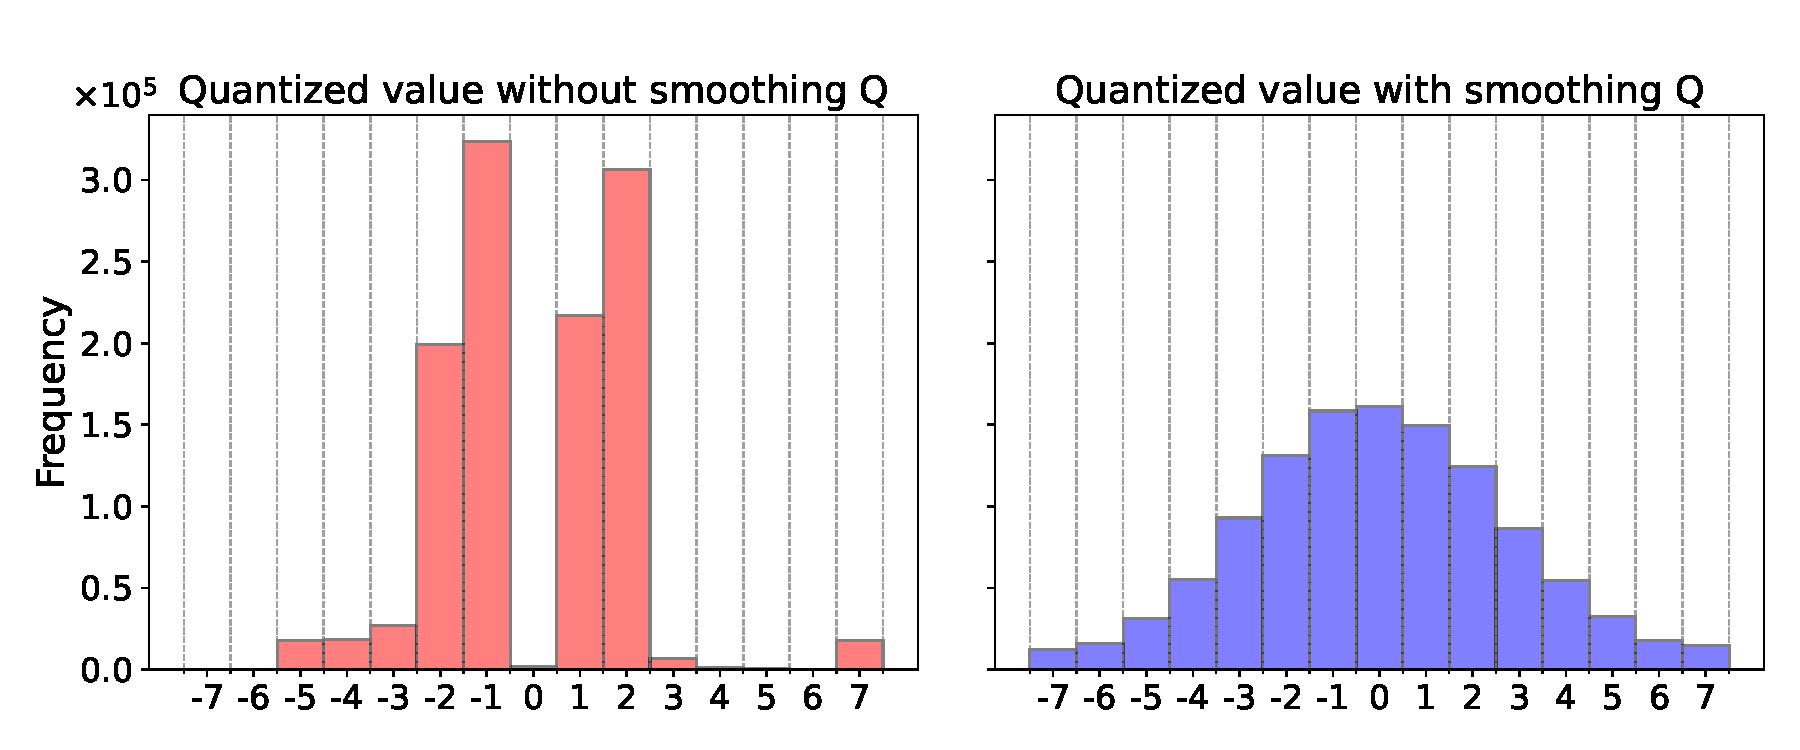
\includegraphics[width=0.72\textwidth]{src/figs/bucket_usage.pdf}
    \vspace{-1em}
    \caption{An example of quantized value distribution of $Q$ before and after smoothing $Q$.}
    \label{fig:bucket_usage}
    \end{center}
\end{figure}



\begin{table*}[h!]
    \centering
    \caption{\textbf{Worst accuracy} across all layers of \cogvideo using different quantization granularities.}
    \label{tab:quant_granularities2}
    \setlength\tabcolsep{13pt}
    \scalebox{1.0}{
    \begin{tabular}{c|c|c|c}
        \toprule
        \textbf{Method} & \textbf{Cos Sim $\uparrow$} & \textbf{Relative L1 $\downarrow$} & \textbf{RMSE $\downarrow$} \\
        \midrule
        Per-token       &  96.76\% & 0.1916 &  0.0775 \\
        Per-thread         & 96.72\% & 0.1932 & 0.0776 \\
        Per-block  &   90.68\%  &  0.3615  &  0.1490  \\
        Per-tensor         & 85.85\% & 0.4687 & 0.2261 \\
        \bottomrule
    \end{tabular}
    }
    \vspace{-1em}
\end{table*}



\begin{table*}[h!]
        \centering
        \caption{\textbf{Worst accuracy} using different data types of $(\widetilde P, V)$ across all layers of a \cogvideo model, where $(Q, K)$ are smoothed.}
        \label{tab:quant_data_type2}
        \setlength\tabcolsep{10pt}
        \scalebox{1.0}{
        \begin{tabular}{c|c|c|c|c}
            \toprule
            $Q, K$ & $\widetilde P, V$ & \textbf{Cos Sim $\uparrow$} & \textbf{Relative L1 $\downarrow$} & \textbf{RMSE $\downarrow$} \\
            \hline
            \multirow{4}{*}{INT4}  & INT8 & \dred{19.52\%} & \dred{0.9579} & \dred{1.4483} \\
                                   & E5M2 & \dred{94.94\%} & \dred{0.2327} & \dred{0.2361} \\
                                   & \bf{E4M3} & \textbf{\dgreen{96.70\%}} & \textbf{\dgreen{0.1956}} & \textbf{\dgreen{0.0779}} \\
                                   & \bf{FP16} & 96.76\% & 0.1916 & 0.0775 \\
            \bottomrule
        \end{tabular}
        }
        \vspace{-1em}
\end{table*}



\begin{table*}[h!]
        \centering
        \caption{\textbf{Worst accuracy} across all layers of \cogvideo using different smooth methods.}
        \label{tab:accuracy_compare2}
        \setlength\tabcolsep{10pt}
        \scalebox{1.0}{
        \begin{tabular}{c|c|c|c}
            \toprule
            \textbf{Method} & \textbf{CosSim $\uparrow$} & \textbf{Relative~L1 $\downarrow$} & \textbf{RMSE $\downarrow$} \\
            \midrule
            None          & 4.83\% & 0.9979 & 0.7784 \\
            \texttt{HadmdAttn}      & 4.85\% & 0.9978 & 0.7785 \\
            \texttt{SmoothAttn}   & 64.49\% & 0.9262 & 0.7204 \\
            \texttt{Smooth K}       & 90.86\% & 0.3565 & 0.1464 \\
            \texttt{Smooth Q}        & 93.10\% & 0.2989 & 0.2195 \\
            \texttt{SageAttn2-4b}   & \textbf{96.71\%} & \textbf{0.1956} & \textbf{0.0779} \\
            \bottomrule
        \end{tabular}}
        \vspace{-1em}
\end{table*}



\begin{table*}[h!]
    \centering
    \begin{minipage}{0.48\linewidth}
        \centering
        \caption{Overhead of per-thread quantization, smoothing Q, and two-level accumulation techniques measured on L20 GPU.}
        \label{tab:ablation_overhead_smoothing}
        \setlength\tabcolsep{18pt}
        \scalebox{1.0}{
        \begin{tabular}{l|c}
            \toprule
            \textbf{Method} & \textbf{TOPS} \\
            \midrule
            Attention (INT4 + FP8) & 284 \\
            + Per-thread quantization & 283 \\
            + Two-level accumulation & 283 \\
            + Smoothing Q & 273 \\
            \bottomrule
        \end{tabular}
        }
    \end{minipage}
    \hfill
    \begin{minipage}{0.48\linewidth}
        \centering
        \caption{Comparison of different quantization granularities measured on L20 GPU, with $QK^\top$ in INT4 and $\widetilde PV$ in FP8.}
        \label{tab:granularity_speed_ablation}
        \setlength\tabcolsep{18pt}
        \scalebox{1.0}{
        \begin{tabular}{l|c}
            \toprule
            \textbf{Granularity} & \textbf{TOPS} \\
            \midrule
            Per-tensor & 286 \\
            Per-block & 284 \\
            Per-thread & 283 \\
            Per-token & 268 \\
            \bottomrule
        \end{tabular}
        }
    \end{minipage}
\end{table*}

\subsection{Additional Experiments and Analysis}  \noindent\textbf{Additional Results.} \label{sec:appendix_analysis_exp}
Table~\ref{exp:metrics_loss_t2t-appendix}, ~\ref{exp:metrics_loss_cogvideo2b-appendix} and ~\ref{exp:metrics_loss_t2t-3_appendix} show results of \our and other baselines on \llama (7B), \cogvideo (2B) and \timm.

\noindent\textbf{Results of Super-Long Context.} We further conduct experiments on super-long context using \texttt{Llama-3-262k} (8B)\footnote{\url{https://huggingface.co/gradientai/Llama-3-8B-Instruct-262k}} on InfiniBench~\cite{zhang-etal-2024-bench} and Needle-in-a-Haystack (NIAH)~\cite{LLMTest_NeedleInAHaystack}, with sequence lengths reaching up to 262k tokens on an H100 GPU. Since Hopper GPUs lack native INT4 tensor core support, we use \texttt{SageAttention2-8b} for this evaluation. We compare it against FlashAttention3(fp8), ensuring both methods operate under the same bit width.
Results are shown in Table~\ref{exp:infinibench_llama3_262k_appendix} and Fig~\ref{fig:llama3_262k_niah}. \our maintains model performance even under super-long context, while FlashAttention3(fp8) suffers from end-to-end accuracy degradation.

\noindent\textbf{Results of Audio Tasks.} We evaluate \texttt{Qwen2-Audio} (7b)~\cite{chu2024qwen2audiotechnicalreport},  a speech-to-text model, on the ASR task using the Librispeech~\cite{Librispeech} test split and measured its performance with the WER metric (Word Error Rate). As shown in Table~\ref{exp:metrics_loss_audio-appendix}, \our consistently outperforms the baselines, highlighting its effectiveness in audio-related models and benchmarks.

\begin{table*}[h!]
    \caption{End-to-end metrics on \texttt{Qwen2-Audio} (7B).}
    \label{exp:metrics_loss_audio-appendix}
    \setlength\tabcolsep{5.5pt}
    \begin{center}
    \scalebox{1.0}{\begin{tabular}{p{2.18cm}|p{3cm}|c|c}
    \toprule
    {\bf Model}  & {\bf Attention}  & {\bf Test-Clean $\downarrow$}  & {\bf Test-Dev $\downarrow$} \\ \hline
    \multirow{6}{*}{\texttt{Qwen2-Audio}} & Full-Precision & 1.74 & 4.01  \\  
    & \texttt{HadmdAttn} & 1.77 &  4.05 \\
    & \texttt{SmoothAttn} & 1.76 &  4.01  \\
    & \texttt{SageAttention} & \textbf{1.74} &  \textbf{4.02}  \\
    & \ourf & \textbf{1.73} &  \textbf{3.99}     \\ 
    & \oure & \textbf{1.72} &  \textbf{4.03}  \\ 
    \bottomrule
    \end{tabular} }
    \end{center}
    \vspace{-1em}
\end{table*}